\documentclass[11pt]{article}
\usepackage[utf8]{luainputenc}
\usepackage[T1]{fontenc}
\usepackage{amsmath,amsfonts,amssymb, amsthm} 
\usepackage{mathtools, thmtools}
\usepackage[onehalfspacing]{setspace}
\usepackage[x11names]{xcolor} 
\usepackage{graphicx}
\usepackage[margin=1in]{geometry}
\usepackage{caption}
\usepackage[pdfencoding=auto, naturalnames, psdextra, colorlinks, citecolor=blue]{hyperref}
\usepackage[noabbrev, capitalise, nameinlink]{cleveref}
\usepackage{csquotes}


\newtheorem{Theorem}{Theorem}[section]
\newtheorem{Corollary}[Theorem]{Corollary}
\newtheorem{Proposition}[Theorem]{Proposition}
\newtheorem{Lemma}{Lemma}[section]

\declaretheorem[style=definition, name=Definition, refname={definition,definitions}, numberwithin=section]{defn}

\usepackage{enumitem}
\newlist{assumplist}{enumerate}{1}
\setlist[assumplist]{label=(\roman{assumplisti}), ref=\roman{assumplisti},noitemsep}

\declaretheorem[style=definition, name=Assumption, refname={assumption,assumptions},
    Refname={Assumption,Assumptions}, numberwithin=section]{assump}
\Crefname{assump}{Assumption}{Assumptions}
\Crefname{assumplisti}{Assumption}{Assumptions}

\addtotheorempostheadhook[assump]{\crefalias{assumplisti}{assump}}
\newcommand*{\fullref}[1]{\hyperref[{#1}]{\namecref{#1} \nameref*{#1}(\labelcref{#1})}}
\newcommand*{\namedref}[1]{\hyperref[{#1}]{\nameref*{#1}(\labelcref{#1})}}
\newcommand*{\Fullref}[1]{\hyperref[{#1}]{\nameCref{#1} \nameref*{#1}(\labelcref{#1})}}


\newcommand{\red}[1]{\textcolor{red}{#1}}
\newcommand{\purple}[1]{\textcolor{purple}{#1}}
\newcommand*{\R}{\mathbb{R}}
\newcommand*{\F}{\mathcal{F}}
\newcommand*{\W}{\mathcal{W}}
\newcommand*{\E}{\mathbb{E}}
\newcommand*{\N}{N}
\newcommand*{\Var}{\mathbb{V}ar}
\newcommand*{\pto}{\ensuremath{\to_p}}
\newcommand*{\dto}{\ensuremath{\to_d}}
\newcommand*{\Eta}{H} 
\newcommand*{\popmom}{\ensuremath{g}} 
\newcommand*{\sampmom}{\ensuremath{\overline{g}_n}}
\DeclarePairedDelimiter\abs{\lvert}{\rvert}
\DeclarePairedDelimiter\norm{\lVert}{\rVert}
\let\oldforall\forall
\let\forall\undefined
\DeclareMathOperator{\forall}{\oldforall}
\DeclareMathOperator{\diag}{diag}
\newcommand{\mvert}[1][\middle]{\ensuremath{\,#1\vert\,}}

\usepackage[backend=biber, autopunct=true, authordate, hyperref=true, doi=false]{biblatex-chicago} 
\addbibresource{riskpriceinference.bib}
\graphicspath{{figures/}}

\author{Xu Cheng, Eric Renault, \& Paul Sangrey}
\title{Inference for the Price of Volatility Risk Under Weak Identification}
\date{\today}

\begin{document}

\maketitle

Two key questions at the very heart of finance are what are the risks investors face and what are the prices of
those risks.
Two leading risks are equity risk and volatility risk.
Although the literature has shown that volatility risk clearly matters, constructing beliefs concerning the price
of volatility risk from the data has proven quite difficult.
What we want is a good estimator for this parameter and a strategy for credible inference regarding it.  

We take the model from \textcite{khrapov2016affine} and use it to estimate the relevant
parameters, which we derive below. 
We use spectral GMM, which forms moment conditions from the characteristic function.
Out data we use are the bivariate series $\begin{pmatrix} r_{t+1}, \sigma^2_{t+1} \end{pmatrix}$.
$r_{t+1}$ is the daily return on some asset, and we use its associated realized volatility for $\sigma^2_{t+1}$.

Moving forward, we sketch the model developed in \textcite{khrapov2016affine} and derive the associated moment
conditions.
We then provide a series of sufficient conditions for valid inference. 
We have a pricing kernel $M_{t, t+1}(\theta)$ which allows us to characterize the price $P_t$ at time $t$ of any
payoff at time $t+1$ of a function $f$ and information set $\F_t$, $f\left(r_{t+1}, \sigma^2(t+1) \mvert
\F_t\right)$. 
We use $*$'s to denote the risk neutral measure.

\begin{equation}
    P_t  = \E\left[M_{t,t+1}(\theta) f\left(r_{t+1}, \sigma^2(t+1) \mvert  \F_t\right) \mvert \F_t \right] =
    \E^{*}\left[H(r_{t+1}, \sigma^2(t+1),  \F_t) \mvert \F_t \right] 
\end{equation}


To make the problem tractable, we assume that the problem is Markov and that there is no Granger causality from
return to volatility. 
This implies the conditional probability distribution of $\sigma^2_{t+1} \vert \F_t$ equals the conditional
probability distribution of $\sigma^2_{t+1} \vert \sigma^2_t$.
Consequently, we can write down our model in the risk-neutral measure using some functions, $a^{*}(u), b^{*}(u)$,
and $\alpha^{*}(v), \phi^{*}(v), \& \gamma^{*}(v)$, as the following two equations in terms of the Laplace
transforms of the probability distributions.

\begin{align}
    \E^{*}\left[\exp\left(-x \cdot \sigma^2_{t+1}\right) \mvert \sigma^2_t\right] &= \exp\left(-a^{*}(x)
    \sigma_t^2 - b^{*}(x)\right) \\
    \E^{*}\left[\exp\left(-x \cdot r_{t+1} \right)\mvert \sigma^2_t \sigma^2_{t+1}\right] &=
    \exp\left(-\alpha^{*}(x) \sigma^2_{t+1} - \phi^{*}(x) \sigma^2_t - \gamma^{*}(x)\right)
\end{align}


\section{The Model}


We assume that the volatility follows an autoregressive gamma process---ARG(1), and so its physical measure
dynamics are governed by following equations.

\begin{gather}
    a(x) = \frac{\rho x}{1 + c x}  \\
    b(x) = \delta \log \left(1 + c x\right) \\
    \rho \in [0, 1), c > 0, \delta > 0 
\end{gather}

The persistence is governed by $\rho$, and the mean by $\delta$, and $c$ is a scaling factor for the volatility as
can be seen in the formula for $\sigma^2_{t+1}$'s conditional mean.

\begin{equation}
    \E\left[\sigma^2_{t+1} \mvert \sigma^2_t\right] = c \delta + \rho \sigma^2_t
\end{equation}

Assuming the measure change preserves the general structure between the risk-neutral and physical measures implies
\cref{eqn:cond_characterisitc_func}.
We also assume that $\left[ \frac{\psi}{\phi} \right]^2 \approx \frac{\E \left[\sigma^2_{t+1} \mvert
\F_t\right]}{\Var\left[r_{t+1} \mvert \F_t\right]}$, which enables our approximation of $\sigma^2_{t+1}$ by the
realized volatility.

\begin{equation}
    \label{eqn:cond_characterisitc_func}
    \E\left[\exp\left(- x \cdot r_{t+1}\right) \mvert \sigma_t^2, \sigma^2_{t+1}\right] = \exp\left(- a(x)
    \alpha^2_{t+1} - \phi(x) \sigma^2_t - \gamma(x) \right) 
\end{equation}

To estimate this equation, we need to know all of the relevant functions.
The parametric structure of the problem and some algebra implies the following.

\begin{align}
    a(x) &= \frac{\rho x}{1 + c x} \\
    b(x) &= \delta \log \left(1 + c x\right) \\
    \alpha(x) &= \psi x - \frac{1}{2} x^2 (1 - \phi^2) \\
    \label{eqn:beta_defn}
    \phi(x)  &= x \alpha^{*}\left(- \frac{\phi}{\sqrt{c [1 + \rho]}} \right) \\
    \label{eqn:gamma_defn}
    \gamma(x) &= x b^{*}\left(- \frac{\phi}{\sqrt{c [1 + \rho]}}\right) 
\end{align}

In last two of the above equations we have the risk-neutral $\alpha^{*}(x)$ and $\phi^{*}(x)$ functions which we
have not defined.
To solve for them we drive the implied stochastic discount factor and make the appropriate measure change.
We parameterize the SDF in terms of price of volatility risk---$\theta_1$---and the price of equity risk---$\theta_2$.
The SDF satisfies the following equation for some functions $m_0(\cdot)$ and $m_1(\cdot)$.

\begin{gather}
    M_{t,t+1}(\theta) = \exp(-r_{f,t}) \exp\left(m_{0}(\theta) + m_1(\theta) \sigma_t^2 - \theta_1 \sigma^2_{t+1}
    - \theta_2 r_{t+1}\right) \\
    \intertext{Then by the law of iterated expectations and some algebra.}
    \E \left[\exp\left(m_{0}(\theta) + m_1(\theta) \sigma_t^2 - \theta_1 \sigma^2_{t+1} - \theta_2 r_{t+1}\right)
    \exp\left(- \alpha(\theta_2) \sigma^2_{t+1} - \phi (\theta_2) \sigma^2_{t+1} - \gamma(\theta_2)\right) \mvert
    \F_t \right] = 1
\end{gather}

This implies the two unspecified functions are as follows.

\begin{align}
    m_{0}(\theta) &= \gamma(\theta_2) + b\left(\alpha\left(\theta_2\right) + \theta_1\right) \\
    m_{1}(\theta) &= \phi(\theta_2) + a\left(\alpha(\theta_2) + \theta_1\right) 
    \intertext{Now we can solve for $\alpha^{*}(x)$ and $\phi^{*}(x)$.}
    a^{*}(x) &= a\left(x + \theta_1 + \alpha(\theta_2)\right) - a\left(\theta_1 + \alpha(\theta_2)\right) \\
    b^{*}(x) &= b\left(x + \theta_1 + \alpha(\theta_2)\right) - b\left(\theta_1 + \alpha(\theta_2)\right) 
\end{align}


We substitute them back into \cref{eqn:beta_defn} and \cref{eqn:gamma_defn} eliminating $\alpha^{*}(x)$ and
$\phi^{*}(x)$.

\begin{align}
    a(x) &= \frac{\rho x}{1 + c x} \\ \label{eqn:a(x)}
    b(x) &= \delta \log \left(1 + c x\right) \\ \label{eqn:b(x)}
    \alpha(x) &= x \left(\frac{\phi}{\sqrt{c (1 + \phi)}}  + (1 - \phi^2)\left(\theta_2 - \frac{1}{2}\right)\right)
    - \frac{1}{2} x^2 (1 - \phi^2) \\ \label{eqn:alpha(x)}
    \phi(x)  &= x \left(a\left(-\frac{\phi}{\sqrt{c(1+ \rho)}} + \theta_1 + \alpha(\theta_2)\right) -
        a\left(\theta_1 + \alpha(\theta_2)\right)\right) \\ \label{eqn:beta(x)}
    \gamma(x) &= x \left(b\left(-\frac{\phi}{\sqrt{c(1+\rho)}} + \theta_1 + \alpha(\theta_2)\right) -
        b\left(\theta_1 + \alpha(\theta_2)\right) \right)
\end{align}


The set of parameters we want to estimate is $\eta \coloneqq \lbrace c, \rho, \delta, \phi, \theta_1,
\theta_2\rbrace$.

\section{Spectral GMM}
\label{sec:spectral_GMM}

We derive a set of moment conditions from the characteristic function above by evaluating it at a grid of points
in $[0,1] \times i [0,1]$. 
That is we can define a function $g_t(x, \eta)$

\begin{equation}
g_t(x, \eta) = Z_t \otimes \begin{bmatrix} \exp(- x \sigma^2_{t+1}) - \exp\left( - a(x) \sigma_t^2 - b(x)
    \right) \\ \exp\left(- x r_{t+1}\right) - \exp\left(- \alpha(x) \sigma^2_{t+1} - \phi(x) \sigma_2^t -
    \gamma(x)\right) \end{bmatrix}
\end{equation}

Where the instruments are given by \cref{eqn:instruments} for complex unit $i$. 

\begin{equation}
    \label{eqn:instruments}
    Z_t = \left[1, \exp\left(- i \sigma_t^2\right), \exp\left(-i \sigma^2_{t-2}\right)\right] 
\end{equation}

The implied unconditional moment restrictions are the following.  

\begin{equation}
    \E \begin{bmatrix}  \mathrm{Re} (g_t(x, \eta)) \\ \mathrm{Im} (g_t(x, \eta)) \end{bmatrix} = 0
\end{equation}


The optimal weighting matrix has its standard form as the precision matrix of the moments as long as we choose a
finite gird for $x$. 
If we use the entire continuum, handling the weights becomes more delicate. 
So we use only finitely many moments for now.
Since the exponential function is a strictly positive function, and we are considering a grid of $x$ values, a
sufficient condition for $\rho, \delta, \& c$ to be identified is for the relevant rows of $\nabla a(x)$ and
$\nabla b(x)$ to equal zero only at $\eta_0$ which are satisfied if $\rho, c, \delta > 0$.
Testing if if $\phi$ and $\theta_2$ are identified is somewhat trickier. 
Consider $\nabla \alpha(x)$. 
%TODO Reword this.
Since we are using a grid of $x$'s, and the gradient of $\alpha$ is a
nonlinear function of $x$, the first two rows of the \cref{eqn:alpha_gradient} imply $\phi$ is identified.

\begin{equation}
    \label{eqn:alpha_gradient}
    \nabla_{\phi, \theta_2, c}  \alpha(x) = \begin{bmatrix} \phi x^{2} + x \left(- 2 \phi \left(\theta_{2} -
    \frac{1}{2}\right) - \frac{\phi}{2 \sqrt{c} \left(\phi + 1\right)^{\frac{3}{2}}} + \frac{1}{\sqrt{c}
    \sqrt{\phi + 1}}\right) \\ x \left(- \phi^{2} + 1\right) \\ \frac{\phi x}{2 c^{\frac{3}{2}} \sqrt{\phi + 1}}
\end{bmatrix} 
\end{equation}

The top line of \cref{eqn:alpha_gradient} can be solved for $\theta_2$, which would create a local lack of
identification for $\theta_2$.
However, this point is ruled out by the other equations.
Consequently,  $\phi \in (-1,1], c > 0$, are sufficient to identify all of the parameters except for $\theta_1$,
the price of volatility risk.

If we plug in the estimated values of the parameters from \textcite{khrapov2016affine} into $\frac{\partial
\phi}{\partial \theta_1}$ and plot it as a function of $\phi$,  we get the following.
The scale is omitted because it is not meaningful. 
As can clearly be seen in \cref{fig:fig:gamma_diff_theta2}, there is a zero when $\phi = 0$.

\begin{figure}[htb]
    \centering
    \caption{Derivative of $\gamma(x)$ with respect to $\theta_2$}
    \label{fig:fig:gamma_diff_theta2}
    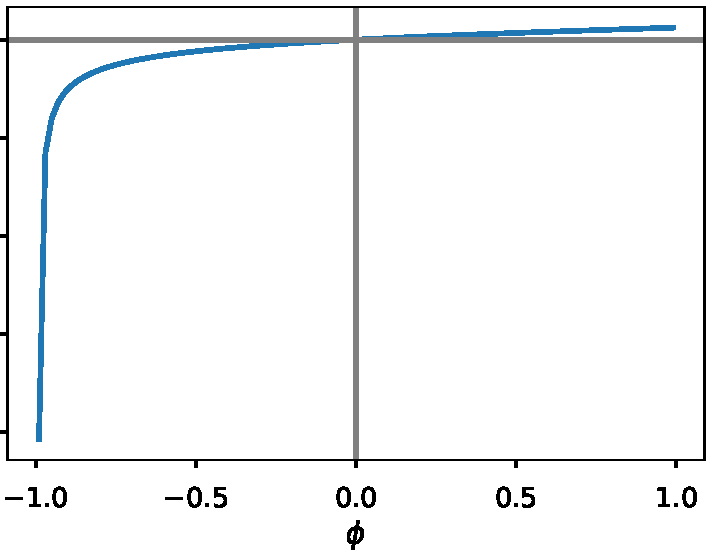
\includegraphics[width=.5\textwidth]{gamma_diff_theta2.pdf}
\end{figure}


For now, we will assume that $\phi \neq 0$, and hence the model is identified.
Hence, for any positive definite weight-matrix by \textcite[Lemma 2.3]{newey1994large} we are identified.
The data, $\sigma^2_{t+1}, r_{t+1}$, are ergodic and stationary.
Since the moment conditions are not redundant the optimal (GMM) weight matrix $W$ is positive definite. 
In addition, $g$ is continuous at each $\eta$, given the restrictions above and properties of characteristic
functions imply that $g$ is uniformly bounded. 
For convenience, we assume that the space of $\eta$ is compact.
This should not be an issue here because the parameters  are either a priori bounded, such as $\phi$ or we have
substantial a priori knowledge on their plausible magnitudes.
Hence, \textcite[Theroem 2.6]{newey1994large} implies our estimator is consistent.

By the above arguments, we have a consistent estimator for $\eta$ and the optimal weight matrix $\eta^{-1}
\coloneqq (\E\left[g g'\right])^{-1}$, and we will assume that $\eta_0$ is in the interior of $\Eta$.
Let $G \coloneqq \E\left[\nabla g\right]$
Clearly, $g$ is continuously differentiable, and its derivative $G$ is continuous.
In addition, by the identification discussion $G' W \nabla G$ is nonsingular.
The only real question is whether $\sqrt{T} g_n(\eta_0) \dto \N(0, \aleph)$ for some positive-definite matrix
$\aleph$.

\begin{assump}[Weak Dependence]
    \label{assumption:weak_dependence}
    $z_t \coloneqq \begin{pmatrix} r_{t+1} \\ \sigma^2_{t+1} \end{pmatrix}$ are $\alpha$-mixing with $\alpha_n =
       O\left(n^{-5}\right)$
\end{assump}

Since, $\norm*{g_n}$ is almost surely bounded by $1$ it has all of its moments and $z_n$ being $\alpha$-mixing
implies $g_n$ is as well by the central limit theorem for strongly mixing process 
$\sqrt{n} g_n(\eta_0) \dto \N(0,\aleph)$ as required. 
Consequently, by \textcite[Theorem 3.2]{newey1994large} we have convergence in distribution as well as convergence
in probability.

\begin{Theorem}[Inference for $\eta$]
    Assume that $\phi  \in (-1,1) \setminus 0$, $\rho \in [0,1)$, and $c > 0$. 
    Further assume that the data are ergodic, stationary, and satisfy \cref{assumption:weak_dependence}.
    Then the following convergence in distribution holds.

    \begin{equation}
        \sqrt{T} (\widehat{\eta}_n - \eta_{0}) \dto \N\left(0, \left(G' \Eta^{-1} G\right)^{-1}\right)
    \end{equation}
\end{Theorem}


\section{Partial Identification Setup}

In this section, take the model described in the previous sections and place it in the setup of
\textcite{andrewsGmm2014} so that we ca analyze the effects of possible lack of identification in the model in a
nice clean way.
The goal here is to perform valid inference for $\theta_1, \theta_2$ even when $\phi$ might be zero. 
To do this effectively, we are going to switch from the notation we were using above to notation used in
\textcite{andrewsGmm2014}. 


From the discussion above, we can collect the parameters discussed above into a parameter vector of the following
form,i.e.\@ recall the following.

\begin{equation}
    \eta \coloneqq \lbrace \rho, c, \delta, \phi, \theta_1, \theta_2 \rbrace
\end{equation}

To write it in the notation of \textcite{andrewsGmm2014}, we partition $\eta$ into three parts.

\begin{align}
    \phi &\coloneqq \phi  \in (-1, 1) \\ 
    \zeta &\coloneqq \lbrace \rho, c, \delta, \theta_1 \rbrace \in [0,1) \otimes \R_{++} \otimes \R_{++} \otimes
    \R  \\
    \pi &\coloneqq \theta_2 \in \R 
\end{align}

Let $\Eta$ be the set of possible $\eta$, that as defined above.
It is worth noting that the parameter space has a product form, i.e.\@ the values do not affect the valid values
of the other parameters.

In this environment, $\pi$ is not identified when $\phi = 0$.
Both $\phi$ and $\zeta$ are always identified.
$\zeta$ does not affect the identification of $\pi$.

Let $Q_n(\eta)$ be the GMM criterion function, then the GMM estimator $\hat{\eta}_n$ satisfies the following.


\begin{equation}
    \hat{\eta}_n \in \Eta\ \text{and}\ Q_n(\hat{\eta}_n) = \inf_{\eta \in \Eta} Q_n(\eta) +
    o\left(n^{-1}\right) 
\end{equation}


Now that we have defined the parameters, we can characterize the set of assumptions necessary for valid inference.
We will work through the assumptions described in \textcite{andrewsGmm2014}.
The set of necessary assumptions is relatively complicated because we have to characterize the asymptotic
distribution under several different estimation strengths simultaneously, and the assumptions required to do that
  differ in the various cases. 
In what follows, we will use 

The first assumption specifies the basic identification
problem. It also provides conditions that are used to determine the
probability limit of the GMM estimator, when it exists, under all categories
of drifting sequences of distributions.
Let $\xi$ index the part of the distribution of the data $x_t$ that is not determined by the moment equations.
In general, it is a (likely infinite-dimensional) nuisance parameter that affects the distribution of the data. 


We collect the parameters that we are estimating $\eta$ and the nuisance parameter $\xi$ into one parameter,
$\gamma$ and associated parameter space $\Gamma$.
In the previous discussion we characterized the parameter spaces in a non-compact fashion, let $\Eta^{*}$ be a
compact subset of $\Eta$, where the true parameter values live.
%TODO Does the set of possible nuisance parameters depend upon the estimated parameters in our model?

\begin{equation}
\Gamma \coloneqq \left\lbrace \gamma = (\eta, \xi) \mvert \eta \in \Eta^{*}, \phi \in \Phi^{*}) \right\rbrace 
\end{equation}

We characterize these drifting sequences of distributions by sequences of true parameters $\gamma_n \coloneqq
(\eta_n, \phi_n)$.

In what follows, three sets of drifting sequences $\lbrace \gamma_n \rbrace$ are key. 

\begin{align}
    \Gamma\left(\gamma_0\right) &\coloneqq \left\lbrace \left\lbrace \gamma_n \in \Gamma \right\rbrace \mvert
        \gamma_n \to \gamma_0 \in \Gamma \right\rbrace\\ 
    \Gamma(\gamma_0, 0, b) &\coloneqq \left\lbrace \lbrace \gamma_n \rbrace \in \Gamma(\gamma_0) \mvert \phi_0 =
        0\ \text{and}\ n^{1/2} \phi_n \to b \in (\R \cup \lbrace \pm \infty) \right\rbrace \\
    \Gamma(\gamma_0, \infty, b_0) &\coloneqq \left\lbrace \lbrace \gamma_n \rbrace \in \Gamma (\gamma_0) \mvert
        n^{1/2} \phi_n \to \infty\ \text{and}\ \phi_n \to b_0 \right\rbrace 
\end{align}


These are the standard GMM regularity conditions appropriately adjusted for the lack of identification when $\phi
=0$.

%TODO
\purple{Question (Xu):}
What is the difference between $g_0\left(\cdot \mvert \gamma_0\right)$ and $g\left(\cdot \mvert \gamma_0\right)$?

\begin{assump}[GMM 1]\label{ass:GMM1}
\begin{assumplist}
    \item If $\phi=0$, $\sampmom(\eta)$ and $\W_{n}(\eta)$ do not depend on $\pi$ for all $\eta \in \Eta$, for
        all $n \geq 1$, and for all $\gamma^{*}\in \Gamma.$ 
        \label{ass:GMM1a}
    \item If $\lbrace \gamma_{n} \rbrace \in \Gamma\left(\gamma_0\right)$, $\sup_{\eta \in \Eta}
        \norm*{\sampmom(\eta) - g_0\left(\eta \mvert \gamma_0\right)} \pto 0$ and $\sup_{\eta
        \in \Eta} \norm{\W_{n}(\eta)-\W\left(\eta \mvert \gamma_0\right)} \pto 0$ for some deterministic
        functions $g_0\left(\eta \mvert \gamma_0\right) : \Eta \times \Gamma \to \R^{k}$ and
        $\W\left(\eta \mvert \gamma_0\right) : \Eta \times \Gamma \to \R^{k\times k}.$
        \label{ass:GMM1b}
    \item When $\phi_0=0$,  $g_0\left(\phi, \zeta ,\pi \mvert \gamma_0\right) = 0$ if and only if $\phi =\phi_0$
        and $\zeta = \zeta_0$ for all $\pi \in \Pi$ and for all $\gamma_0 \in \Gamma.$
        \label{ass:GMM1c}
    \item When $\phi_0 \neq 0$, $g_0\left(\eta \mvert \gamma_0\right)=0$ if and only if $\eta =\eta_0$ for all 
        $\gamma_0 \in \Gamma.$
        \label{ass:GMM1d}
    \item  $g_0\left(\eta \mvert \gamma_0\right)$ is continuously differentiable in $\eta $ on $\Eta$ with partial
        derivatives with respect to $\theta$ and $\xi$ denoted by $g_{\eta }\left(\theta \mvert
        \gamma_0\right) \in R^{k\times d_{\eta }}$ and $g_{\xi }\left(\eta \mvert \gamma_0\right)\in R^{k\times
        d_{\xi }}$, respectively.
        \label{ass:GMM1e}
    \item $\W\left(\eta \mvert \gamma_0\right)$ is continuous in $\eta$ on $\Eta$ for all $\gamma_0\in \Gamma$.
        \label{ass:GMM1f}
    \item $0 < \lambda_{\min}(\W\left(\xi_0, \pi \mvert \gamma_0\right))\leq \lambda_{\max }(\W\left(\xi_0,\pi
        \mvert \gamma_0\right)) < \infty$, $\forall \pi \in \Pi$, for all $\gamma_0 \in \Gamma$.
        \label{ass:GMM1g}
    \item $\lambda_{\min} (g_{\xi}\left(\xi_0,\pi \mvert \gamma_0\right)^{\prime} \W\left(\xi_0,\pi \mvert
        \gamma_0\right)g_{\xi }\left(\xi_0,\pi \mvert \gamma_0\right))>0$, for all $\pi \in \Pi$,  and for all 
        $\gamma_0 \in \Gamma$ with $\phi_0=0.$
        \label{ass:GMM1h}
    \item$\Xi(\pi)$ is compact for all $\pi \in \Pi$, and both $\Pi$ and $\Eta$ are compact.
        \label{ass:GMM1i}
    \item For all $\epsilon > 0$, there exits a $\delta > 0$ such that $d_{H}\left(\Xi \left(\pi_{1}\right), \Xi
        \left( \pi_{2}\right) \right) < \epsilon$ for $\pi_{1}, \pi_{2} \in \Pi$ with $\norm*{\pi_{1}-\pi_{2}} <
        \delta$, where $d_{H}\left( \cdot \right)$ is the Hausdorff metric.
        \label{ass:GMM1j}
\end{assumplist}
\end{assump}

To verify the conditions above, we break them down into three subsections.
Assumptions \namedref{ass:GMM1a}, \namedref{ass:GMM1b}, \namedref{ass:GMM1c}, and \namedref{ass:GMM1d}
state that when $\phi = 0$, the moment conditions contain no information regarding $\pi$, but when $\phi \neq 0$,
the model is identified.

%TODO
\purple{TODO (Paul): 
Relate those assumptions to the discussion in \cref{sec:spectral_GMM}
We need to show that \namedref{ass:GMM1b} holds; we showed it holds pointwise in \cref{sec:spectral_GMM} but not
in a functional sense. (At least I think so.)}

The next two assumptions (\namedref{ass:GMM1e} and \namedref{ass:GMM1f} are  technical conditions regarding the
behavior of the moment conditions and weight matrix. 
%TODO
\purple{TODO: (Paul) Is this true?} 
Since our moment conditions are derived from an infinitely-differentiable  characteristic function and the weight
matrix is the optimal one, they both hold trivially.

The third subsection of Assumption \nameref{ass:GMM1} concerns the weight matrix.
Since we are using the inverse covariance matrix of valid non-redundant model, assumptions \namedref{ass:GMM1g}
and \namedref{ass:GMM1h} automatically hold.

The last two assumptions, \namedref{ass:GMM1i} and \namedref{ass:GMM1j} require that the parameter spaces do not
vary too much with the parameters and are compact.
Since the parameter space here has a product form, \namedref{ass:GMM1j}  holds trivially.
\namedref{ass:GMM1i} does not hold.
However, since there exists compact sets that contain the parameters---Even the parameters whose domain is
theoretically unbounded have bounds on the apriori believable
estimates---and $(\phi, \zeta)$ are identified this is not an issue in practice. 


%TODO
\purple{Question: (Xu) What is $\Eta_n(\delta_n)$. Is the domain the same in \namedref{ass:GMM2b} and
\namedref{ass:GMM2c}?}


\begin{assump}[GMM 2*]\label{ass:GMM2}
\begin{assumplist}
    \item $\sampmom(\eta)$ is continuously differentiable in $\eta$ for all $n \geq 1$. 
        \label{ass:GMM2a}
    \item If $\{\gamma_n\} \in \Gamma\left(\gamma_0, 0, b\right)$, $\sup_{\left\lbrace \eta \in \Eta
        \mvert \norm*{(\phi, \zeta')' - (\phi, \zeta')_{0,n}'} \leq \delta_n \right\rbrace}
        \norm*{\frac{\partial}{\partial \xi'} \sampmom(\eta) - \popmom_{\xi}\left(\eta \mvert \gamma_0 \right)} =
        o_p(1)$  for all deterministic sequences  $\delta_n \to 0$.
        \label{ass:GMM2b}
    \item If $\{\gamma_n \} \in \Gamma\left(\gamma_0, \infty, \eta_0\right)$, $\sup_{\eta \in \Eta_{n}(\delta_n)}
        \norm*{\left(\frac{\partial}{\partial \eta'} \overline{g}_n - g_{\eta}\left(\eta \mvert
        \gamma_0\right)\right) \diag\left(1_{1+d_\zeta}', (1/\phi_n)_{d_{\pi}}'\right)}  = o_p(1)$ for all
        deterministic sequences $\delta_n \to 0$.
        \label{ass:GMM2c}
\end{assumplist}
\end{assump}


Since our moment conditions are sample average of the characteristic function, they satisfy \namedref{ass:GMM2a}
automatically. 
%TODO
\purple{TODO: We need to show that \namedref{ass:GMM2b} and \namedref{ass:GMM2c} are satisfied (they are) using a
uniform law of large numbers and the dominated convergence theorem.}
\textcite{andrewsGmm2014} show that this is a sufficient condition for their Assumption GMM2, which is what we
actually need. 

Once we have \nameref{ass:GMM1} and \nameref{ass:GMM2}, we use \nameref{ass:GMM3} to derive the asymptotic
distribution under weak and semi-strong identification.
These conditions will be characterized using the expected derivative of the population moment conditions. 


\begin{defn}
    \label{defn:moment_derivative_func}
    \begin{equation}
        K_{n,g}\left(\eta \mvert \gamma^{*}\right) \coloneqq  \frac{1}{n} \sum_{i=1}^n \frac{\partial}{\partial
        \phi^{*}} \E \left[ \popmom(W_i, \eta) \mvert \gamma^{*} \right]
    \end{equation}
\end{defn}


\begin{assump}[GMM 3]\label{ass:GMM3}
\begin{assumplist}
    \item $\sampmom(\eta) = \frac{1}{n} \sum_{i=1}^n \popmom(W_i, \eta)$  for some function $\popmom(W_i,
        \eta) : \R^{k \times k} \times \Eta \to \R^k$.
        \label{ass:GMM3a}
    \item $\E\left[\popmom(W_i, \beta_0, \zeta^{*}, \pi) \mvert \gamma^{*} \right] = 0$ for all $\pi \in \Pi$ and
        for all $i \geq 1$ if $\gamma^{*} = \left(0,\zeta^{*}, \pi^{*}, \xi^{*} \right) \in \Gamma$.
        \label{ass:GMM3b}
    \item If $\{ \gamma_n \} \in \Gamma(\gamma_0, 0, b)$, $\frac{1}{\sqrt{n}} \sum_{i=1}^n \left(g(W_i,
        \zeta_{0,n}, \pi_n) - \E \left[g(W_i, \zeta_{0,n}, \pi_n)\mvert \gamma_n \right]\right)  \dto \N\left(0,
        \aleph_g(\gamma_0)\right)$, where $\aleph_{g}(\gamma_0)$ is a $k \times k$ matrix.
        \label{ass:GMM3c}
    \item 
        \label{ass:GMM3d}
        \begin{enumerate}
            \item  $K_{n,g}\left(\eta \mvert \gamma^{*}\right)$ exists for all $\{\eta, \gamma^{*} \} \in
                \left(\Eta_{\delta} \times \Gamma_{0}\right)$ and for all $n \geq 1$.
            %TODO
            \item[] \purple{Question (Xu): What is $\tilde{\gamma}$, i.e.\@ why does $\gamma$ have a tilde when
                the other parameters do not?}
            \item $K_{n,g}\left(\phi_n, \zeta_n, \pi \mvert \tilde{\gamma}_n\right)$ uniformly converges to some
                non-stochastic matrix-valued function  $K_{g}\left(0, \zeta_0, \pi \mvert \gamma_0\right)$  over
                $\pi \in \Pi$ for all deterministic sequences $\{\phi_n, \zeta_n, \tilde{\gamma}_n \}$ satisfying
                $\tilde{\gamma}_n \in \Gamma$, $\tilde{\gamma_n} \to \gamma_0 \coloneqq (0, \zeta_0, \pi_0, \xi)$,
                $\{\phi_n, \zeta_n, \pi \} \in \Eta$ and $\{\phi_n, \zeta_n \} \to (0, \zeta_0)$.
            \item $K_g\left(\phi_0, \zeta_0, \pi \mvert \gamma_0\right)$ is continuous on $\Pi$ for all  $\gamma_0
                \in \Gamma$ with $\phi_0 = 0$.
        \end{enumerate}
        \item $K\left(\phi_0, \zeta_0, \pi \mvert \gamma_0\right) = \popmom_{\phi, \zeta}\left(\phi_0, \pi\mvert
            \gamma_0\right) x$ for some $x \in \R^{1+d_{\zeta}}$ if and only $\pi = \pi_0$.\footnote{Since
                $\dim(\phi) = 1$, we can assume without loss of generality that the $\omega_0$ from
            \textcite{andrewsGmm2014} equals $1$.}
        \label{ass:GMM3e}
        %TODO
        \item[] \purple{Question (Xu): What is the difference between $g(W_i, \eta)$ evaluated at $\eta = \eta_n$
            and $g(W_i, \eta_n)$?}
        \item If $\{ \gamma_n \} \in \Gamma(\gamma_0, 0, b)$, $\left. \frac{1}{n} \sum_{i=1}^n
            \frac{\partial}{\partial \eta}  \E \left[ \popmom\left(W_i, \eta\right ) \mvert \gamma_n \right]
            \right\rvert_{\eta = \eta_n} \to \popmom_{\eta}\left(\eta_0 \mvert \gamma_0\right)$.
        \label{ass:GMM3f}
\end{assumplist}
\end{assump}

Assumption \namedref{ass:GMM3a} is trivially satisifed,  and we showed that \namedref{ass:GMM3b} is satisfied in
\cref{sec:spectral_GMM}.
%TODO
\purple{TODO: Show that \nameref{ass:GMM3c} is sasfied by using a triangular CLT}


First, start by defining $g^{*}$ as follows, where (as used above) $g_{x}$ refers to the derivative of $g$ with
respect to $x$.
Note, assumptions \namedref{ass:GMM1a} and \namedref{ass:GMM3a}  imply that when $\phi_0 = 0$,
$g_{\zeta}\left(\phi_0, \zeta_0, \pi \mvert \gamma_0\right)$, does not depend upon $\pi$.


\begin{defn}{\popmom*}
    \begin{equation}
        g_{\phi, \zeta}^{*}\left(\phi_0, \zeta_0, \pi_1, \pi_2 \mvert \gamma_0\right)  =
        \left[g_{\phi}\left(\phi_0, \zeta_0, \pi_1 \mvert \gamma_0\right)  , g_{\phi}\left(\phi_0, \zeta_0, \pi_2
        \mvert \gamma_0\right) , g_{\zeta} \left(\phi_0, \zeta_0 \mvert \gamma_0\right)  \right]  \in \R^{k \times
        (d_{\zeta} + 2)}
    \end{equation}
\end{defn}

\begin{assump}[GMM 4]\label{ass:GMM4}
\begin{assumplist}
    \item $\phi$ is a scalar.
    \item $g_{\phi, \zeta}^{*}\left(\phi_0, \zeta_0, \pi_1, \pi_2 \mvert \gamma_0\right)$ has full column rank. 
    \item $\aleph_g(\gamma_0)$ is positive definite for all $\gamma_0 \in \gamma $ with $\phi_0 = 0$. 
\end{assumplist}
\end{assump}





\printbibliography





\end{document}


